\section{Ejercicios del libro}

\subsubsection*{Ejercicio 11}

Use la Regla del Punto Medio con el valor dado de \( n \) para aproximar la integral. Redondee cada respuesta a cuatro decimales.


\[
9. \quad \int_{0}^{10} \sin \sqrt{x} \,dx, \quad n = 5
\]

\[
x_i = a + \Delta x \cdot i
\]

\[
x_{i-1} = a + \Delta x (i-1)
\]

\[
x_i^* = \frac{x_i + x_{i-1}}{2}
\]

\[
x_i^* = \frac{a + \Delta x \cdot i + a + \Delta x (i-1)}{2}
\]


\[
x_i^* = \frac{2a + (2i-1) \Delta x}{2}
\]

\[
x_i^* = a + \frac{2i -1}{2} \Delta x
\]

\[
x_i^* = a + \left(i - \frac{1}{2} \right) \Delta x
\]

\[
\Delta x = \frac{10}{5} = 2
\]

\[
x_i^* = \left(i - \frac{1}{2} \right) 2 = 2i -1
\]

\[
f(x_i^*) = \sin \sqrt{2i -1}
\]

\[
A = k \sum_{i=1}^{n} f(x_i^*)
\]

\[
A = 2 \sum_{i=1}^{10} \sin \sqrt{2i -1}
\]


\[
A = 2 \left[ \sin \sqrt{1} + \sin \sqrt{3} + \sin \sqrt{5} + \sin \sqrt{7} + \sin \sqrt{9} \right]
\]

\[
A = 6.4643 \, u^2
\]


\subsubsection*{Ejercicio 13}

Si tiene un sistema algebraico computacional (CAS) que evalúa aproximaciones por punto medio y grafica los rectángulos correspondientes (use los comandos \texttt{middlesum} y \texttt{middlebox} en Maple), verifique la respuesta del Ejercicio 11 e ilustre con un gráfico. Luego, repita con \( n = 20 \) y \( n = 30 \).

Usando MATLAB, se obtienen las siguientes gráficas:

\[
\text{Para } n = 5; \quad f(x) = \sin(\sqrt{x})
\]

\begin{figure}[H]
    \centering
    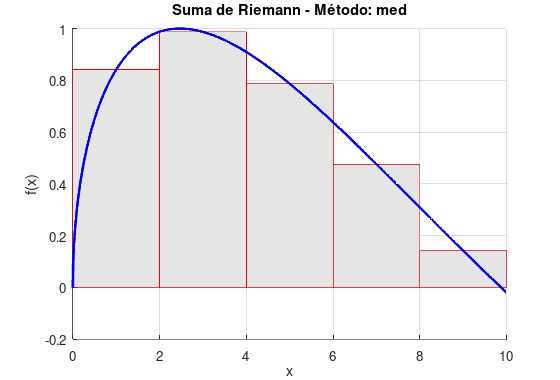
\includegraphics[scale=0.5]{images/1 n5.jpeg}
    \label{fig:riemann_med}
\end{figure}

\[
\text{Aproximación de la integral (med): } 6.464277
\]


\[
\text{Para } n = 20; \quad f(x) = \sin(\sqrt{x})
\]

\begin{figure}[H]
    \centering
    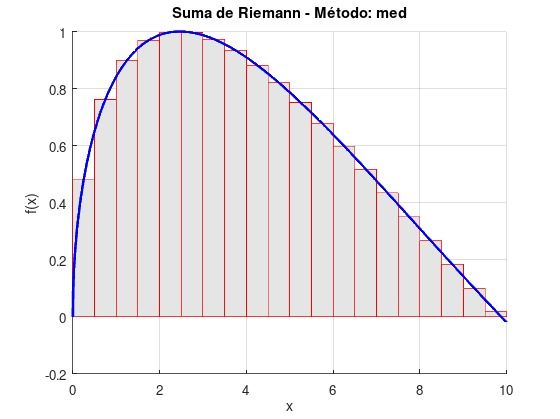
\includegraphics[scale=0.5]{images/2 n20.jpeg}
    \label{fig:riemann_med_n20}
\end{figure}

\[
\text{Aproximación de la integral (med): } 6.304519
\]


\[
\text{Para } n = 30; \quad f(x) = \sin(\sqrt{x})
\]

\begin{figure}[H]
    \centering
    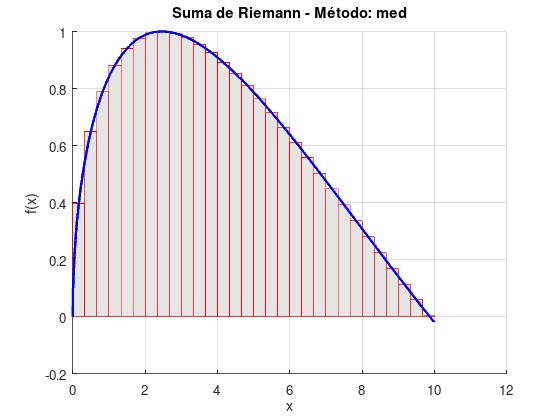
\includegraphics[scale=0.5]{images/3 n30.jpeg}
    \label{fig:riemann_med_n30}
\end{figure}

\[
\text{Aproximación de la integral (med): } 6.294108
\]

Puede acceder al script de MATLAB en el siguiente enlace: \url{https://github.com/johanP051/tareaII-calculoII/blob/main/latex/analisisComputacional/cas.m}

\subsubsection*{Ejercicio 17}

Expresar el límite como una integral definida en el intervalo dado.


\[
\lim_{n \to \infty} \sum_{i=1}^{n} x_i \sin x_i \Delta x, \quad [0, \pi]
\]

\[
= \int_{0}^{\pi} (x \sin x) \,dx
\]

\textbf{Usando integración por partes:}

\[
\int x \sin x \,dx
\]

\[
\text{Sea } u = x, \quad dv = \sin x \,dx
\]

\[
du = dx, \quad v = -\cos x
\]

Aplicando la fórmula de integración por partes:

\[
\int u dv = uv - \int v du
\]

\[
\int x \sin x \,dx = -x \cos x + \int \cos x \,dx
\]

\[
\int x \sin x \,dx = -x \cos x + \sin x
\]

Evaluamos en los límites de integración:

\[
\int_{0}^{\pi} x \sin x \,dx = \left[ -x \cos x + \sin x \right]_{0}^{\pi}
\]

\[
= \left( -\pi \cos \pi + \sin \pi \right) - \left( -0 \cos 0 + \sin 0 \right)
\]

\[
= (-\pi (-1) + 0) - (0 + 0)
\]

\[
= \pi
\]

\subsubsection*{Ejercicio 19}

\[
\lim_{n \to \infty} \sum_{i=1}^{n} \left[ 2(x_i^*)^2 - 5x_i^* \right] \Delta x, \quad [0,1]
\]

\[
= \int_{0}^{1} (5x^2 - 5x) \,dx
\]

\[
= \int_{0}^{1} 5x(x - 1) \,dx
\]

\subsubsection*{Ejercicio 21}

\[
\int_{-1}^{5} (1 + 3x) \,dx
\]

\[
= \int_{-1}^{5} dx + \int_{-1}^{5} 3x \,dx
\]

\[
= \left[ x \right]_{-1}^{5} + \left[ \frac{3}{2} x^2 \right]_{-1}^{5}
\]

\[
= (5 - (-1)) + \frac{3}{2} \left( 5^2 - (-1)^2 \right)
\]

\[
= 6 + \frac{3}{2} \cdot 24
\]

\[
= 6 + 36
\]

\[
= 42
\]


\subsubsection*{Ejercicio 23}

\[
\int_{0}^{2} (2 - x^2) \,dx
\]

\[
= \left[ 2x - \frac{1}{3}x^3 \right]_{0}^{2}
\]

\[
= 2(2) - \frac{1}{3} (2^3)
\]

\[
= 4 - \frac{8}{3}
\]

\[
= \frac{8}{3}
\]

\subsubsection*{Ejercicio 25}

\[
\int_{1}^{2} x^3 \,dx
\]

\[
= \left[ \frac{1}{4} x^4 \right]_{1}^{2}
\]

\[
= \frac{1}{4} \left[ 2^4 - 1^4 \right]
\]

\[
= \frac{1}{4} \left[ 16 - 1 \right]
\]

\[
= \frac{15}{4}
\]


\subsubsection*{Ejercicio 27}

\[
\int_{0}^{\pi} \sin 5x \,dx
\]

\[
x_i = \frac{\pi}{n} i
\]

\[
\lim_{n \to \infty} \sum_{i=1}^{n} \frac{\pi}{n} \sin \left( \frac{5\pi}{n} i \right)
\]

\textbf{Resolviendo la integral:}

Sabemos que:

\[
\frac{d}{dx} \cos(ax) = -a \sin(ax)
\]

Por lo que:

\[
\int -a \sin(ax) \,dx = a \int -\sin(ax) \,dx
\]

\[
= a \frac{\cos(ax)}{a}
\]

\[
= \cos(ax)
\]

Aplicamos esta propiedad a la integral dada:

\[
\int_{0}^{\pi} \sin(5x) \,dx = \left[ \frac{-\cos(5x)}{5} \right]_{0}^{\pi}
\]

\[
= \frac{-\cos(5\pi)}{5} - \frac{-\cos(0)}{5}
\]

\[
= \frac{-(-1)}{5} - \frac{-1}{5}
\]

\[
= \frac{1 + 1}{5} = \frac{2}{5} = 0.2
\]

\subsubsection*{Ejercicio 29}

\textbf{Se muestra la gráfica de \( f \). Evalúe cada integral interpretándola en términos de áreas.}

\begin{enumerate}[label=(\alph*)]
    \item \( \int_{0}^{2} f(x) \,dx \)
    \item \( \int_{0}^{5} f(x) \,dx \)
    \item \( \int_{5}^{7} f(x) \,dx \)
    \item \( \int_{0}^{9} f(x) \,dx \)
\end{enumerate}

\begin{figure}[H]
    \centering
    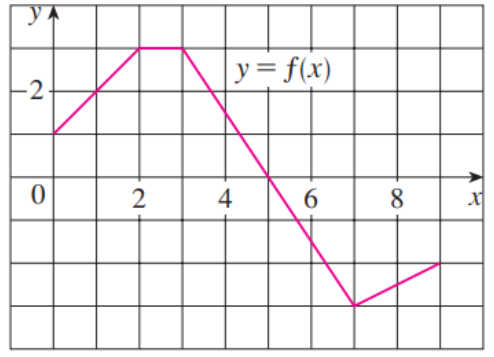
\includegraphics[scale=0.3]{images/integral1.png}
\end{figure}

\[
\text{(a)} \quad \int_{0}^{2} f(x)\,dx 
= \frac{3 + 1}{2} \cdot 2 
= 4
\]

\begin{figure}[H]
    \centering
    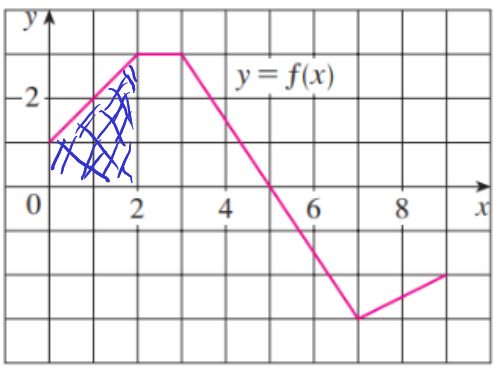
\includegraphics[scale=0.3]{images/integral2.png}
\end{figure}

\[
\text{(b)} \quad \int_{0}^{5} f(x)\,dx 
= \int_{0}^{2} f(x)\,dx \;+\; \int_{2}^{5} f(x)\,dx 
= 4 \;+\; \frac{3 + 1}{2} \cdot 3 
= 10
\]

\begin{figure}[H]
    \centering
    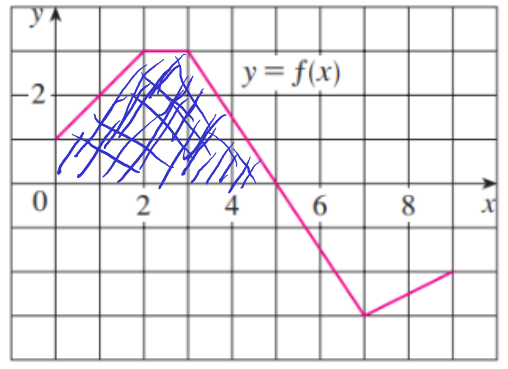
\includegraphics[scale=0.3]{images/integral3.png}
\end{figure}

\[
\text{(c)} \quad \int_{5}^{7} f(x)\,dx 
= \frac{2(-3)}{2} = -3
\]

\begin{figure}[H]
    \centering
    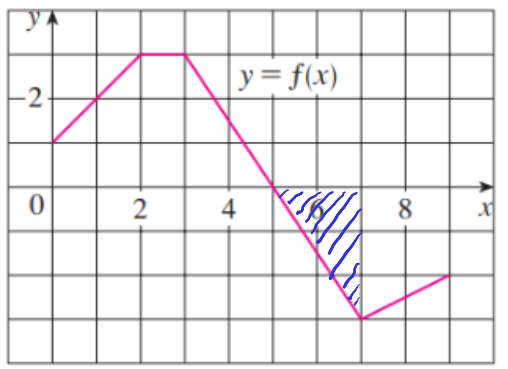
\includegraphics[scale=0.3]{images/integral4.png}
\end{figure}

\[
\text{(d)} \quad \int_{0}^{9} f(x)\,dx 
= \int_{0}^{5} f(x)\,dx + \int_{5}^{7} f(x)\,dx + \int_{7}^{9} f(x)\,dx
\]

\[
= 10 - 3 - \frac{3+2}{2} \cdot 2
\]

\[
= 10 - 3 - 5
\]

\[
= 2
\]

\begin{figure}[H]
    \centering
    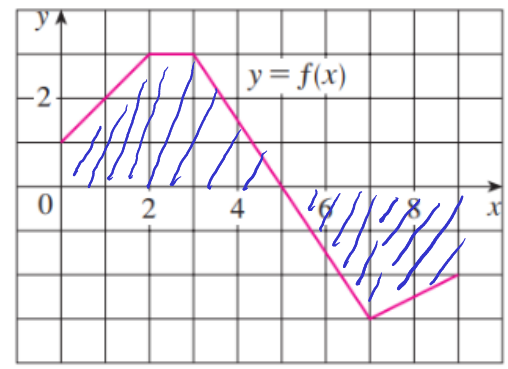
\includegraphics[scale=0.3]{images/integral5.png}
\end{figure}

\subsubsection*{Ejercicio 31}

\[
\quad \int_{1}^{3} (1 + 2x) \,dx
\]

\[
= \int_{1}^{3} 1 \,dx + \int_{1}^{3} 2x \,dx
\]

\[
= \left[ x \right]_{1}^{3} + 2 \left[ \frac{x^2}{2} \right]_{1}^{3}
\]

\[
= (3 - 1) + \left( 3^2 - 1^2 \right)
\]

\[
= 2 + 8
\]

\[
= 10
\]
